\iffalse

\bibliography{..\\bib\\tex.bib}

\fi

\chapter{Word Embedding 模型的介绍}
\label{chap:w2v}

\emph{The Distributional Hypothesis}告诉我们:``words which are similar in meaning occur in similar contexts''\citep{rubenstein1965contextual},即具有相似意义的词语也会出现在相似的环境中。基于这个假设,我们可以设计一个在学习时评价词向量好坏的标准\mydash 通过某个词语来预测出现这个词语的语言环境的准确度,或通过某个语言环境来预测中心词语的准确度。例如,对于一组词向量,如果可以使用这组词向量很准确地通过中心词来预测上下文的话,我们就认为这组词向量较好地符合了\emph{The Distribtuional Hypothesis},同时也会具有较高的质量。下面我们对包括\emph{word2vec}在内的几个模型进行介绍。

在下面的介绍中,我们将训练语料记为$D$,他的大小为$|D|$,我们将他的第$i$个词语标记为$w_i$,对应的字典为$W$,字典的大小为$|W|$,将第$i$个词语的词向量标记为$\vvec_i$,每个词向量的维度为$N$

\section{N-Gram模型}

N-Gram模型假设语料中每个词语出现的概率,只取决于那个词语之前的$n-1$个词语,而与其他任何信息都没有关系。我们也可以理解为这种模型将每个词语出现位置前的$n-1$个词语作为词语的上下文,并试图通过上下文来预测词语。

N-Gram模型中,比较成功的是\cite{bengio2006neural},这个模型设计了一个三层的神经网络来对N-Gram模型进行建模。第一层的神经网络将词语的编号$w_i$转换为对应的向量$\vvec_i$,第二层的神经网络通过第$i$个词语的前$n-1$个词语,$w_{i-n+1}, ... , w_{i-1}$,计算第$i$个词语的上下文对应向量$\vecc = g(w_{i-n+1}, ..., w_{i-1})$,最后一层通过第$i$个词语的上下文对应的向量通过soft-max函数计算第$i$个词语出现的概率:
\begin{eqnarray*}
&&P(w_i| w_{i-n+1}, ..., w_{i-1}) \\
&=& P(w_i | \vecc) \\
&=& \frac{e^{\vecc_{w_i}}}{\sum_j e^{\vecc_{w_j}}}
\end{eqnarray*}
其中:
\begin{eqnarray*}
\vecc = b + W\vvec + U \mathrm{tanh}(d+H\vvec) \\
\vvec = [\vvec_{i-n+1}, ..., \vvec{i-1}]
\end{eqnarray*}

这样设计的神经网络,由于共享词向量,可以认为是自带平滑效果的。例如,即使在$D$中``A dog is sleeping''出现的次数远大于``A cat is sleeping'',由于``dog''和``cat''的词向量非常相似,这两个句子的概率并不会有太大的差异。在实际实验中,这个模型的实验结果也确实要比精心设计了平滑项的n-gram算法要好$10\%$到$20\%$

\section{SENNA模型}
\label{sec:senna}
在\cite{bengio2006neural}的模型中,词向量只是作为N-Gram模型的一个组件,一个部分。实际上,词向量可以在自然语言处理领域的多种任务中均起到非常重要的作用。\cite{collobert2011natural}所提出的SENNA模型就并不关注如何描述文本,或如何计算$P(w_i|w_{i-n+1}, ..., w_{i-1})$,而是如何以词向量为桥梁进行自然语言处理领域的多项任务。SENNA模型在计算出词向量后,会将词向量运用在许多自然语言领域的其他任务中继续训练,并达成类似多任务学习的效果。由于我们在这里更关心词向量的学习,所以我们仅介绍他学习词向量的方法。

区别于N-Gram模型,SENNA刻画的并不是$P(w_i|w_{i-n+1}, ..., w_{i-1})$,而是$P(w_i, w_{i-n+1}, ..., w_{i-1})$即连续$n$个词语出现的概率,他将这个概率看作由这$n$个词语构成的句子的自然程度,并记做$f(w_i, w_{i-1}, ..., w_{i-n+1}) = g(w_{\frac{2i-n-1}{2}})$。虽然$f$被解释为概率,但实际在训练的时候,$f$并没有被当作概率来进行训练,而是单纯得当成了一个度量句子质量(自然程度)的函数。同时,在训练的时候,所优化的目标为:

\begin{eqnarray}
\label{eq:senna}
\sum_{\{w_i, ..., w_{i-n+1}\} \in D} \sum_{w^* \in W} max\{0, 1 - g(w_{\frac{2i-n-1}{2}}) + g(w^*) \}
\end{eqnarray}

其中$g(w^*)$表示将包含连续n个词语的句子的中间的词语换为字典中任意一个单词$w^*$后所得句子的自然程度。可以看到,式\ref{eq:senna}可以被理解成一个以max-margin作为损失函数的判别一个句子中间词的分类器,这个分类器将除去中间词的其余词作为中间词的语言环境,并将替换掉中间词后的句子作为负例。

\section{\emph{word2vec}的模型}

前面所介绍的模型中,N-Gram模型将第$i$个词的前$n-1$个词作为第$i$个词的语言环境,并通过预测第$i$个词提高训练词向量。SENNA模型可以理解为将第$i$个词的周围$n-1$个词作为第$i$个词的语言环境,并通过预测第$i$个词来训练词向量,可以看到词向量的语言环境由前面的词语变成了周围的词语,直观地看,后者应该是更为合理的。另一方面,在词向量使用上,N-Gram模型只是将词向量作为文本输入的方式来克服维度灾难,并获得额外的模型平滑。而SENNA模型,则将词向量做为了更重要的部件,她将词向量单独进行训练,并将其作为连接自然语言处理多个任务的枢纽。

下面我将要介绍的\emph{word2vec}模型则是一个专门的对于词向量进行学习的工具。他将第i个词语周围的$n$个词语作为这个词语的上下文,并通过两种方式设计目标函数,来进行词向量的学习。同时通过词向量本身与简单的相似度计算的算法,就可以在一些基础的自然语言处理问题达到不错的效果。

\emph{word2vec}有两种设计目标函数的方式,同时也有两种对模型的计算进行简化的方式,我们下面对他们进行一一介绍。

\subsection{Skip-gram模型与CBOW模型}

如同上文所说,\emph{word2vec}的模型都是将第$i$个词的周围$n$个词作为其上下文或语言环境,但是他们却有两种建模方式,简单来说,一种是通过词来预测语言环境,称为Skip-gram,一种是通过语言环境来预测词,称为Continuous Bag-of-Words(CBOW)。下面我们分别对他们进行介绍。

\subsubsection{Skip-gram模型}

\begin{figure}
\centering
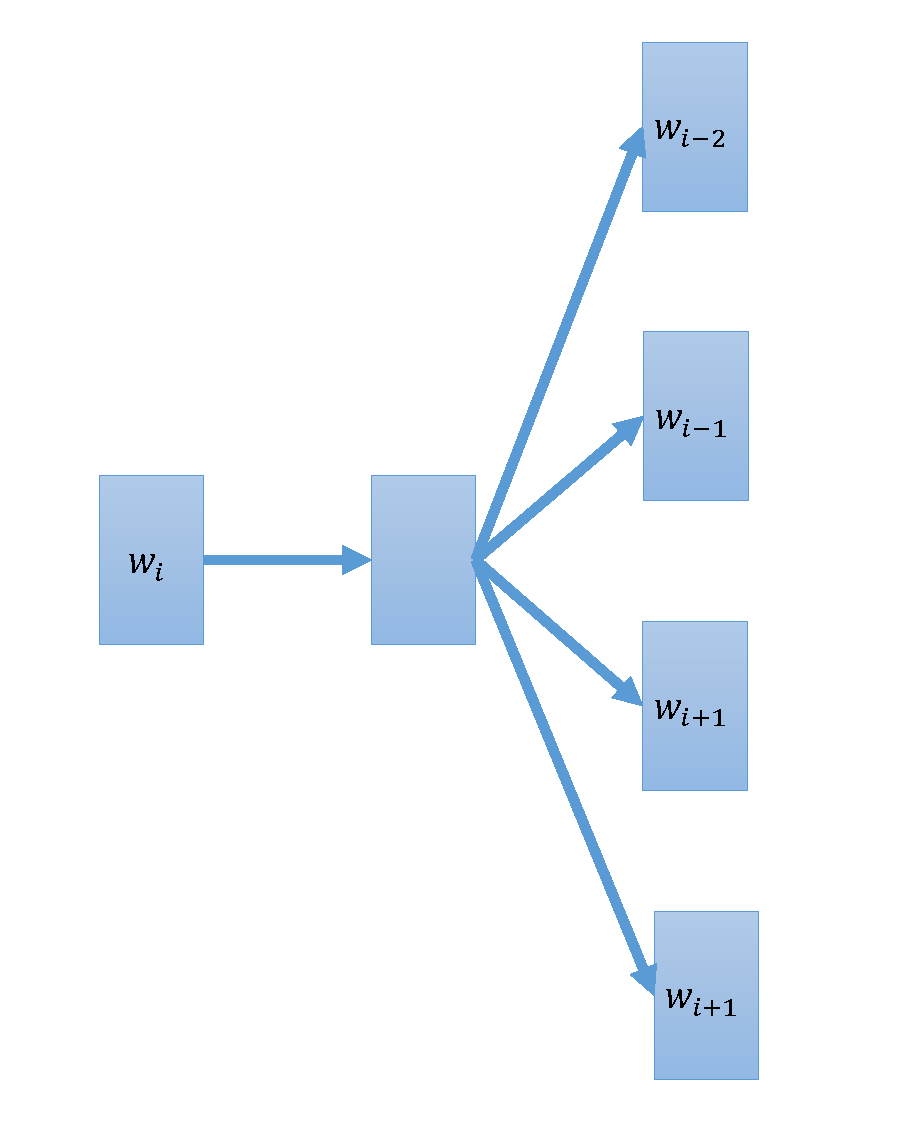
\includegraphics[width=7cm]{skip_gram}
\caption{当$n=4$时Skip-gram网络结构示意图}
\label{fig:skip_gram}
\end{figure}

如\ref{fig:skip_gram}所示,Skip-gram模型由一个两层的神经网络组成,第一层将$w_i$转化为对应的词向量$\vvec_i$,第二层通过soft根据获得的词向量预测$w_i$的上下文,即$w_{i-2}, w_{i-1}, w_{i+1}, w_{i+2}$,需要注意的是,Skip-gram模型并不考虑上下文所包含词语的顺序,即将上下文当作一个集合,而不是列表。Skip-gram模型的目标函数为:
\begin{eqnarray*}
\sum_{w_i \in D} \sum_{-\frac{n}{2}\leq j \frac{n}{2}} \mathrm{log}P(w_{i+j} | w_i)
\end{eqnarray*}
其中$P(w_{i+j} | w_i)$表示了由一个词语预测其上下文的概率模型。基础版本的$P(w_{i+j} | w_i)$是通过soft-max函数实现的: 
\begin{equation}
\label{eq:soft_max}
P(w_O | w_I) = \frac{e^{{\vvec'_O}^\top \vvec_I}}{\sum_{j \in W} e^{{\vvec'_j}^\top \vvec_I}}
\end{equation}
其中$w_i$与$w'_i$分别表示输入与输出的词向量表示。事实上这个最基础的soft-max版本并不能很好得直接运用在实际运算中。这主要是因为一般情况下,字典都会有较大量级的词语,而基础的soft-max的梯度计算的开销是正比于词向量中变量的个数的。我们会在后面看到,\emph{word2vec}提出了两种可以以较高效率进行计算的soft-max的近似。

\subsubsection{CBOW模型}

\begin{figure}
\centering
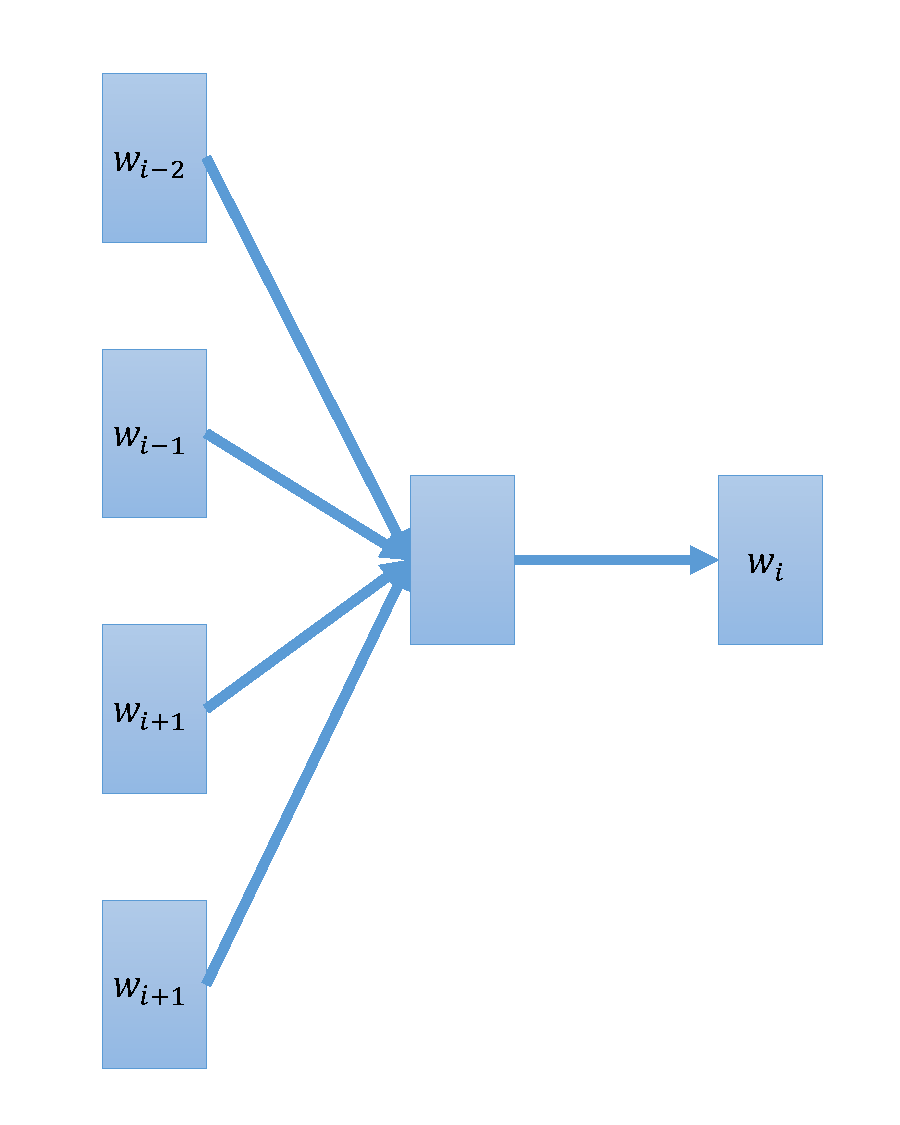
\includegraphics[width=7cm]{CBOW}
\caption{当$n=4$时CBOW网络结构示意图}
\label{fig:CBOW}
\end{figure}

CBOW模型区别于Skip-gram模型之处在于,他是通过根据一个词的语言环境/上下文预测这个词来训练词向量的。同时,CBOW模型是一个词袋模型,即他将第$i$个词的周围n个词看作一个词袋,只关心他们在没在这个词袋中出现,而不关心他们在这个词袋中的位置与顺序。与skip-gram模型类似,CBOW的模型同样是一个两层的神经网络,如\ref{fig:CBOW}所示,第一层将某个词语的上下文的词语转化为对应得向量并将他们的和作为上下文对应的语言环境向量,第二层根据这个语言环境向量预测这个词语到底是哪一个。他的目标函数为:
\begin{eqnarray*}
\sum_{w_i \in D} \mathrm{log}P(w_{i} | \sum_{-\frac{n}{2}\leq j \frac{n}{2}} \vvec_{i+j})
\end{eqnarray*}

其中的函数$P$如式\ref{eq:soft_max}一样,也是soft-max函数,这里就不再赘述。

\subsection{Hierarchical Softmax与Negative Sampling}

如上文所说,如果直接使用soft-max函数计算$P(w_O | w_I)$会带来性能上的缺陷与瓶颈。为了简化计算,\emph{word2vec}提出了两种近似方式:Hierarchical Softmax与Negative Sampling。我们下面分别对他们进行介绍。

\subsubsection{Hierarchical Softmax}

最基础的soft-max函数,即使只需要计算某个词语出现的概率,都要使用包含在$W$中的每个词语对应的词向量(共$|W|\cdot N$个变量)来计算正规化项,这需要进行大量的运算。实际上,soft-max函数中运算需求最大的地方就是正规化项。为了简化soft-max,最直观的思路就是改变soft-max的计算方式,使得她的正规化不需要非常大量的计算。\cite{morin2005hierarchical}使用名为Hierarchical Softmax的树状的结构网络,改变了soft-max的计算方式,使之只需要约$\mathrm{log}_2(|W|)$个维度为$N$的向量既可计算出某个词语出现的概率。

具体来说,这个网络将字典中的词语进行编码,并将对应的二叉编码树的结构移植到输出层。这时,该模型假设输出层的每个叶子节点都代表一个词语,而由根节点出发随机游走到达某叶子节点的概率就等于对应词语出现的概率。比如说,对于单词$w$,由于网络的输出层为一棵二叉树,所以有且仅有一条从根节点出发的路径可以到达$w$对应得叶子节点。我们将从根节点出发的这条路径的长度记为$L(w)$,路径上的第$j$个点记为$n_w^j)$,其中$n_w^1)$为root, $n_w^{L(w)}$为w。则由hierarchical softmax计算出的$P(w_O | w_I)$为:
\begin{equation}
\label{eq:HS}
P(w | w_I) = \prod_{j = 1}^{L(w) - 1} \sigma(\mathrm{if}(n_w^{j+1} = \mathrm{ch}_{(n(w,j))})\cdot {\vvec'_{n_w^j}}^\top \vvec_{w_I})
\end{equation}
其中$\sigma(x) = \frac{1}{1+e^{-x}}$为sigmoid激励函数,$if(x)$在$x$为真时为1,$x$为假时为-1,$\mathrm{ch}_(n)$为n的一个子节点。通过证明,我们知道,$\sum_{w \in W} P(w | w_I) = 1$,即在使用上述定义计算$P(w | w_I)$时,不需要额外进行正规化的计算。这使得hierarchical softmax的函数及微分计算均正比于$L(w_O)$,而不是$|W|$。

\subsubsection{Negative Sampling}

除去Hierarchical Softmax,另一种\emph{word2vec}所介绍的对于soft-max进行简化的方式被称为Negative Sampling。类似于\ref{sec:senna}中所介绍的SENNA模型,由于\emph{word2vec}实际上并不关心skip-gram模型或CBOW模型所进行预测的准确度,而是希望通过他们,可以学习到具有高质量的词向量。Negative Sampling就是基于soft-max函数设计出的一种可以度量词向量质量的函数。他将基于soft-max的目标函数中的$\mathrm{log}P(W_{O}|W_{I})$替换为:
\begin{equation}
\label{eq:NS}
\mathrm{log}\sigma({\vvec'_{w_O}}^\top\vvec_{w_I}) + \sum_{i = 1}^k \mathbb{E}_{w_i \sim P_n(w)}[\mathrm{log}\sigma(-{\vvec'_{w_i}}^\top\vvec_{w_I})]
\end{equation}

这种构造可以被直观得理解为构造负例,然后再试图将正例与负例之间的差异最大化。同时,另一方面,如同我们已经在\ref{sec:word2vecmf}中提到过的一样,这种构造负例的方法,可以被理解为是在一种特殊的信息矩阵上进行矩阵分解。这些分析与讨论也为Negative Sampling提供了理论依据。同时,在验证试验中,\emph{Negative Sampling}也有很好的实际表现。在下面的文章中,我们也将会将\emph{word2vec}模型作为讨论的重点。